\begin{comment}
What was good/bad about the implementation?
 - Initial design was too simple, and didn’t account for various complexities in the what was required for Open MCT and other sources
 - DB design: Was this good? Could it be done better after making changes to how Open MCT best works with data?

What worked, and what didn’t?
\end{comment}

\section{Results and Discussion}
The latest version of the source code for the implemented system is available at \url{https://github.com/NTNU-SmallSat-Lab/hypso-openmct}. Release version 1.0 is the subject of the results and discussion in the rest of this report unless otherwise is specified. The documentation for version 1.0 is also included in appendix C.

\begin{figure}[ht]
  \centering
  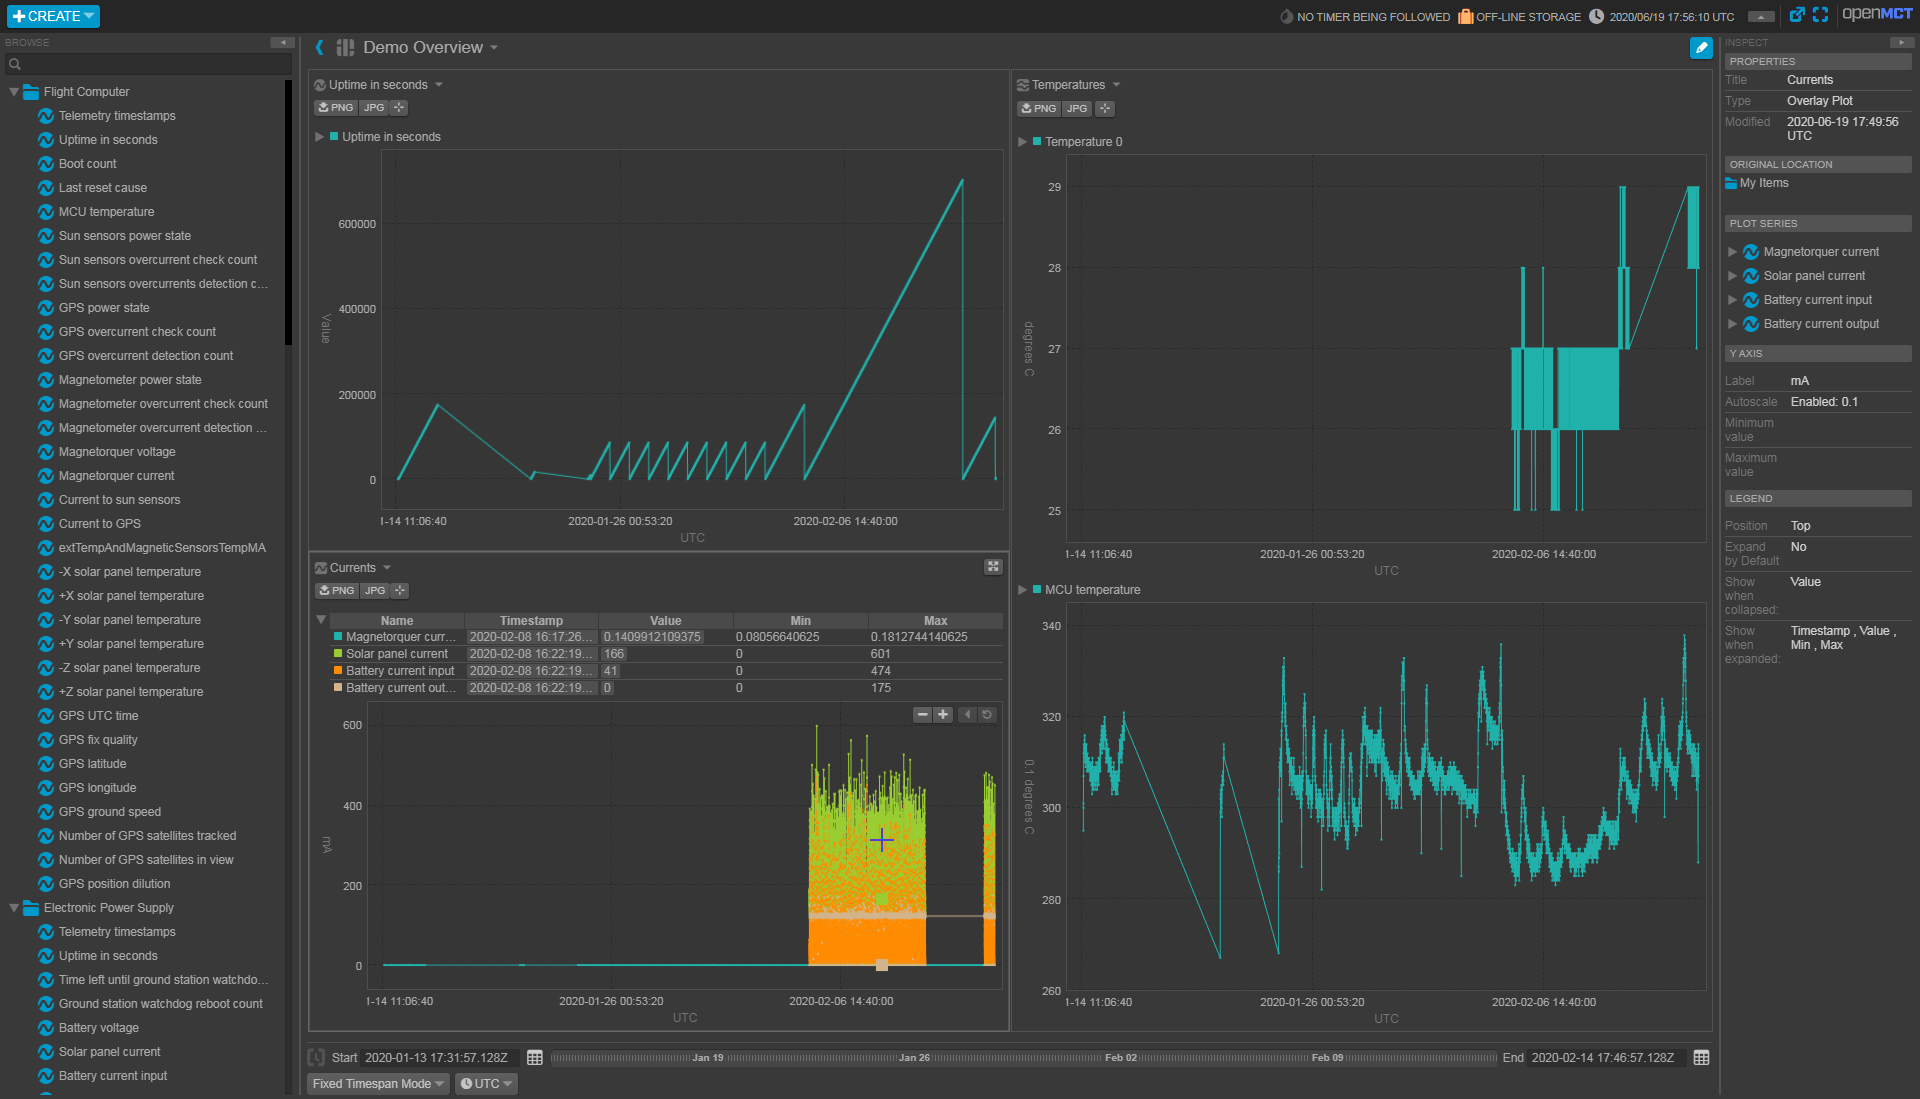
\includegraphics[width=1\linewidth]{Images/Demo Overview.png}
  \caption{Sample Open MCT view}
  \label{fig:demoview}
\end{figure}

The v1.0 release allows viewing of historical and realtime telemetry data for the HYPSO satellite Electrical Power Supply and Flight Computer, with a custom sample view of this data shown in Figure \ref{fig:demoview}. This data may currently be loaded from a JSON file exported from the \acrshort{na} \Gls{postgrest} API, and in theory by connecting the server directly to the \Gls{postgrest} API, although this has only been tested against a mock server due to time and computer access constraints.

\subsection{Design change summary}
All of the modules in the system required some level of change or adaptation during development. Certain classes (such those for the logger and payload controller telemetry) were removed from version 1.0 due to insufficient time or test data, while others (such as the \inlinecode{DbPoller} and \inlinecode{DbHasher}) were added to account for unplanned changes in the implementation.

The telemetry serving and client subsystems in particular were not described in much detail in the design draft, and have had multiple new classes added, such as a new \acrshort{http} server-client pair for providing system configuration and telemetry metadata to Open MCT.

The database-related classes also saw multiple changes due to the initial specification for them being too simple or slow in practice.

A more detailed description of the changes and the reasoning behind them may be found below.

\subsection{Final system architecture}
An overview of the class diagram for the implemented system may be found in Figure \ref{fig:new_class}. Attempting to read this directly is again not recommended due to its size, and it is mostly included as a way to get a quick overview of the connections between the subsystems.

\begin{sidewaysfigure}[ht]
  \centering
  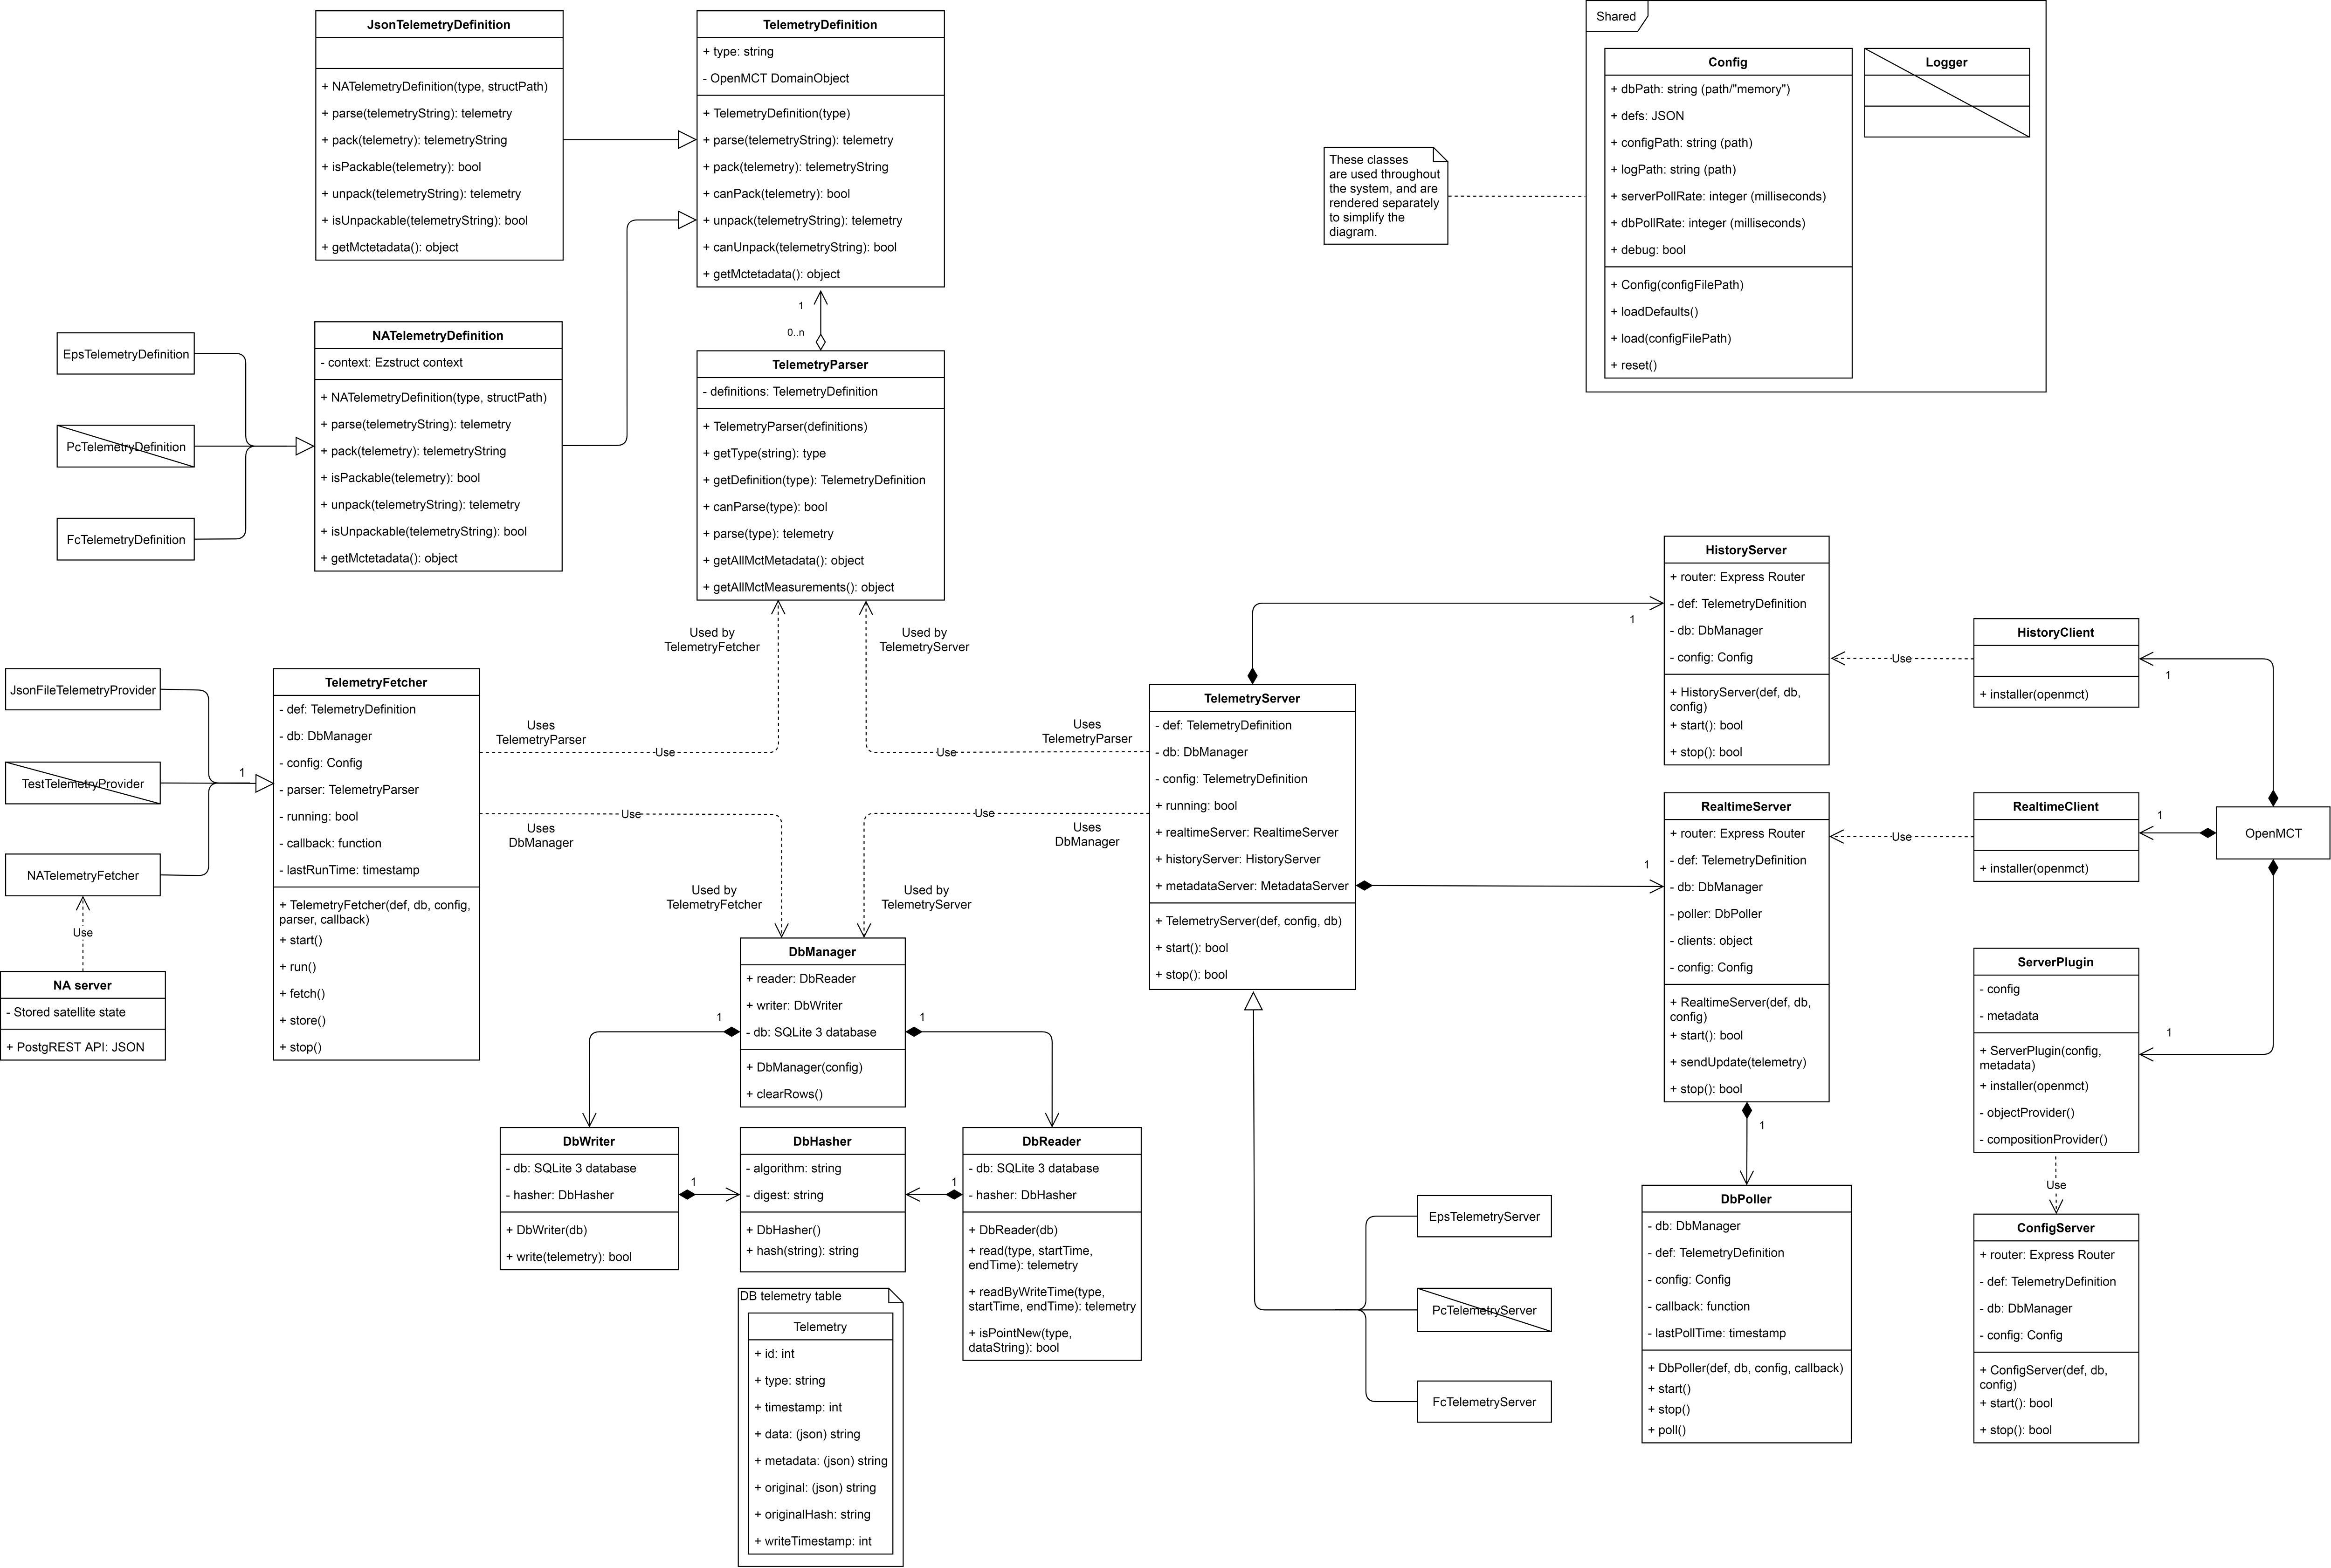
\includegraphics[width=1\linewidth]{Images/New Diagrams/Class Diagram Large.png}
  \caption{New Class Diagram Overview}
  \label{fig:new_class}
\end{sidewaysfigure}

\subsubsection{Shared modules}
The \inlinecode{Config} class did not see any major changes except for the removal of the methods for exporting the configuration, as these were not found to be particularly useful in practice for version 1.0.

The \inlinecode{Logger} class was removed due to lack of time to properly implement it.

The updated class diagram for these modules can be found in Figure \ref{fig:new_cdshared}.

\begin{figure}[H]
  \centering
  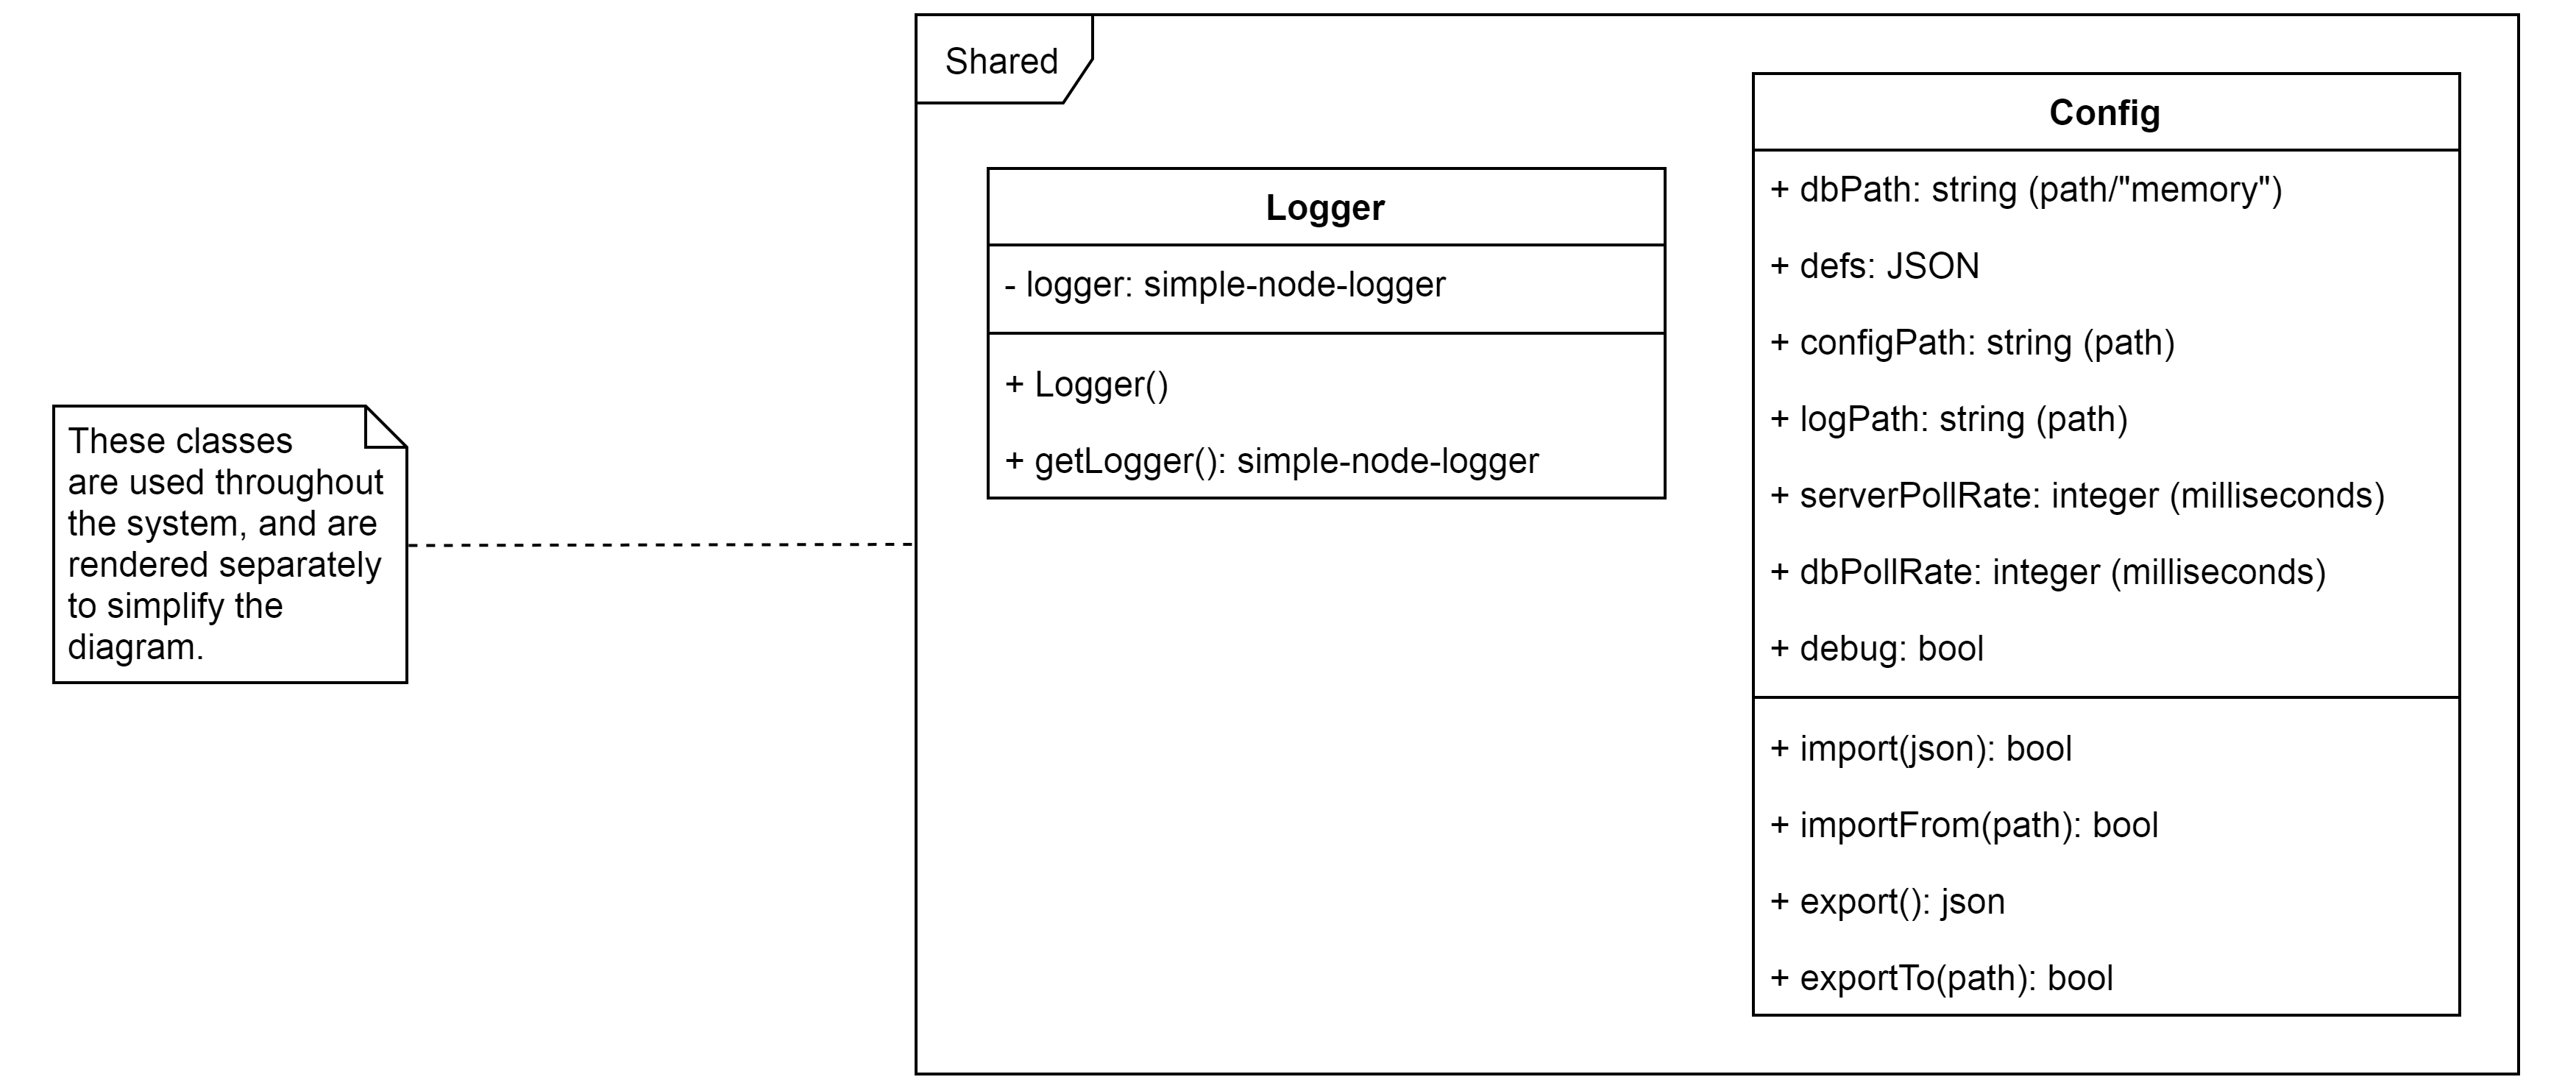
\includegraphics[width=0.75\linewidth]{Images/New Diagrams/SharedModules.png}
  \caption{New Class Diagram: Shared Modules}
  \label{fig:new_cdshared}
\end{figure}

\subsubsection{Telemetry fetching subsystem}
The main changes in the \inlinecode{TelemetryFetcher} class is the \inlinecode{fetch()} method being split into \inlinecode{run()} (which calls the following methods at regular intervals), \inlinecode{fetch()} (which gets and parses data from a given telemetry source) and \inlinecode{store()} (which stores the parsed data if it isn't in the database already). This was done to decouple the running and storing steps from the fetching process, to make it easier to only redefine the methods required when adding a new telemetry source.

The updated class diagram for these modules can be found in Figure \ref{fig:new_cdfetching}.

\begin{figure}[H]
  \centering
  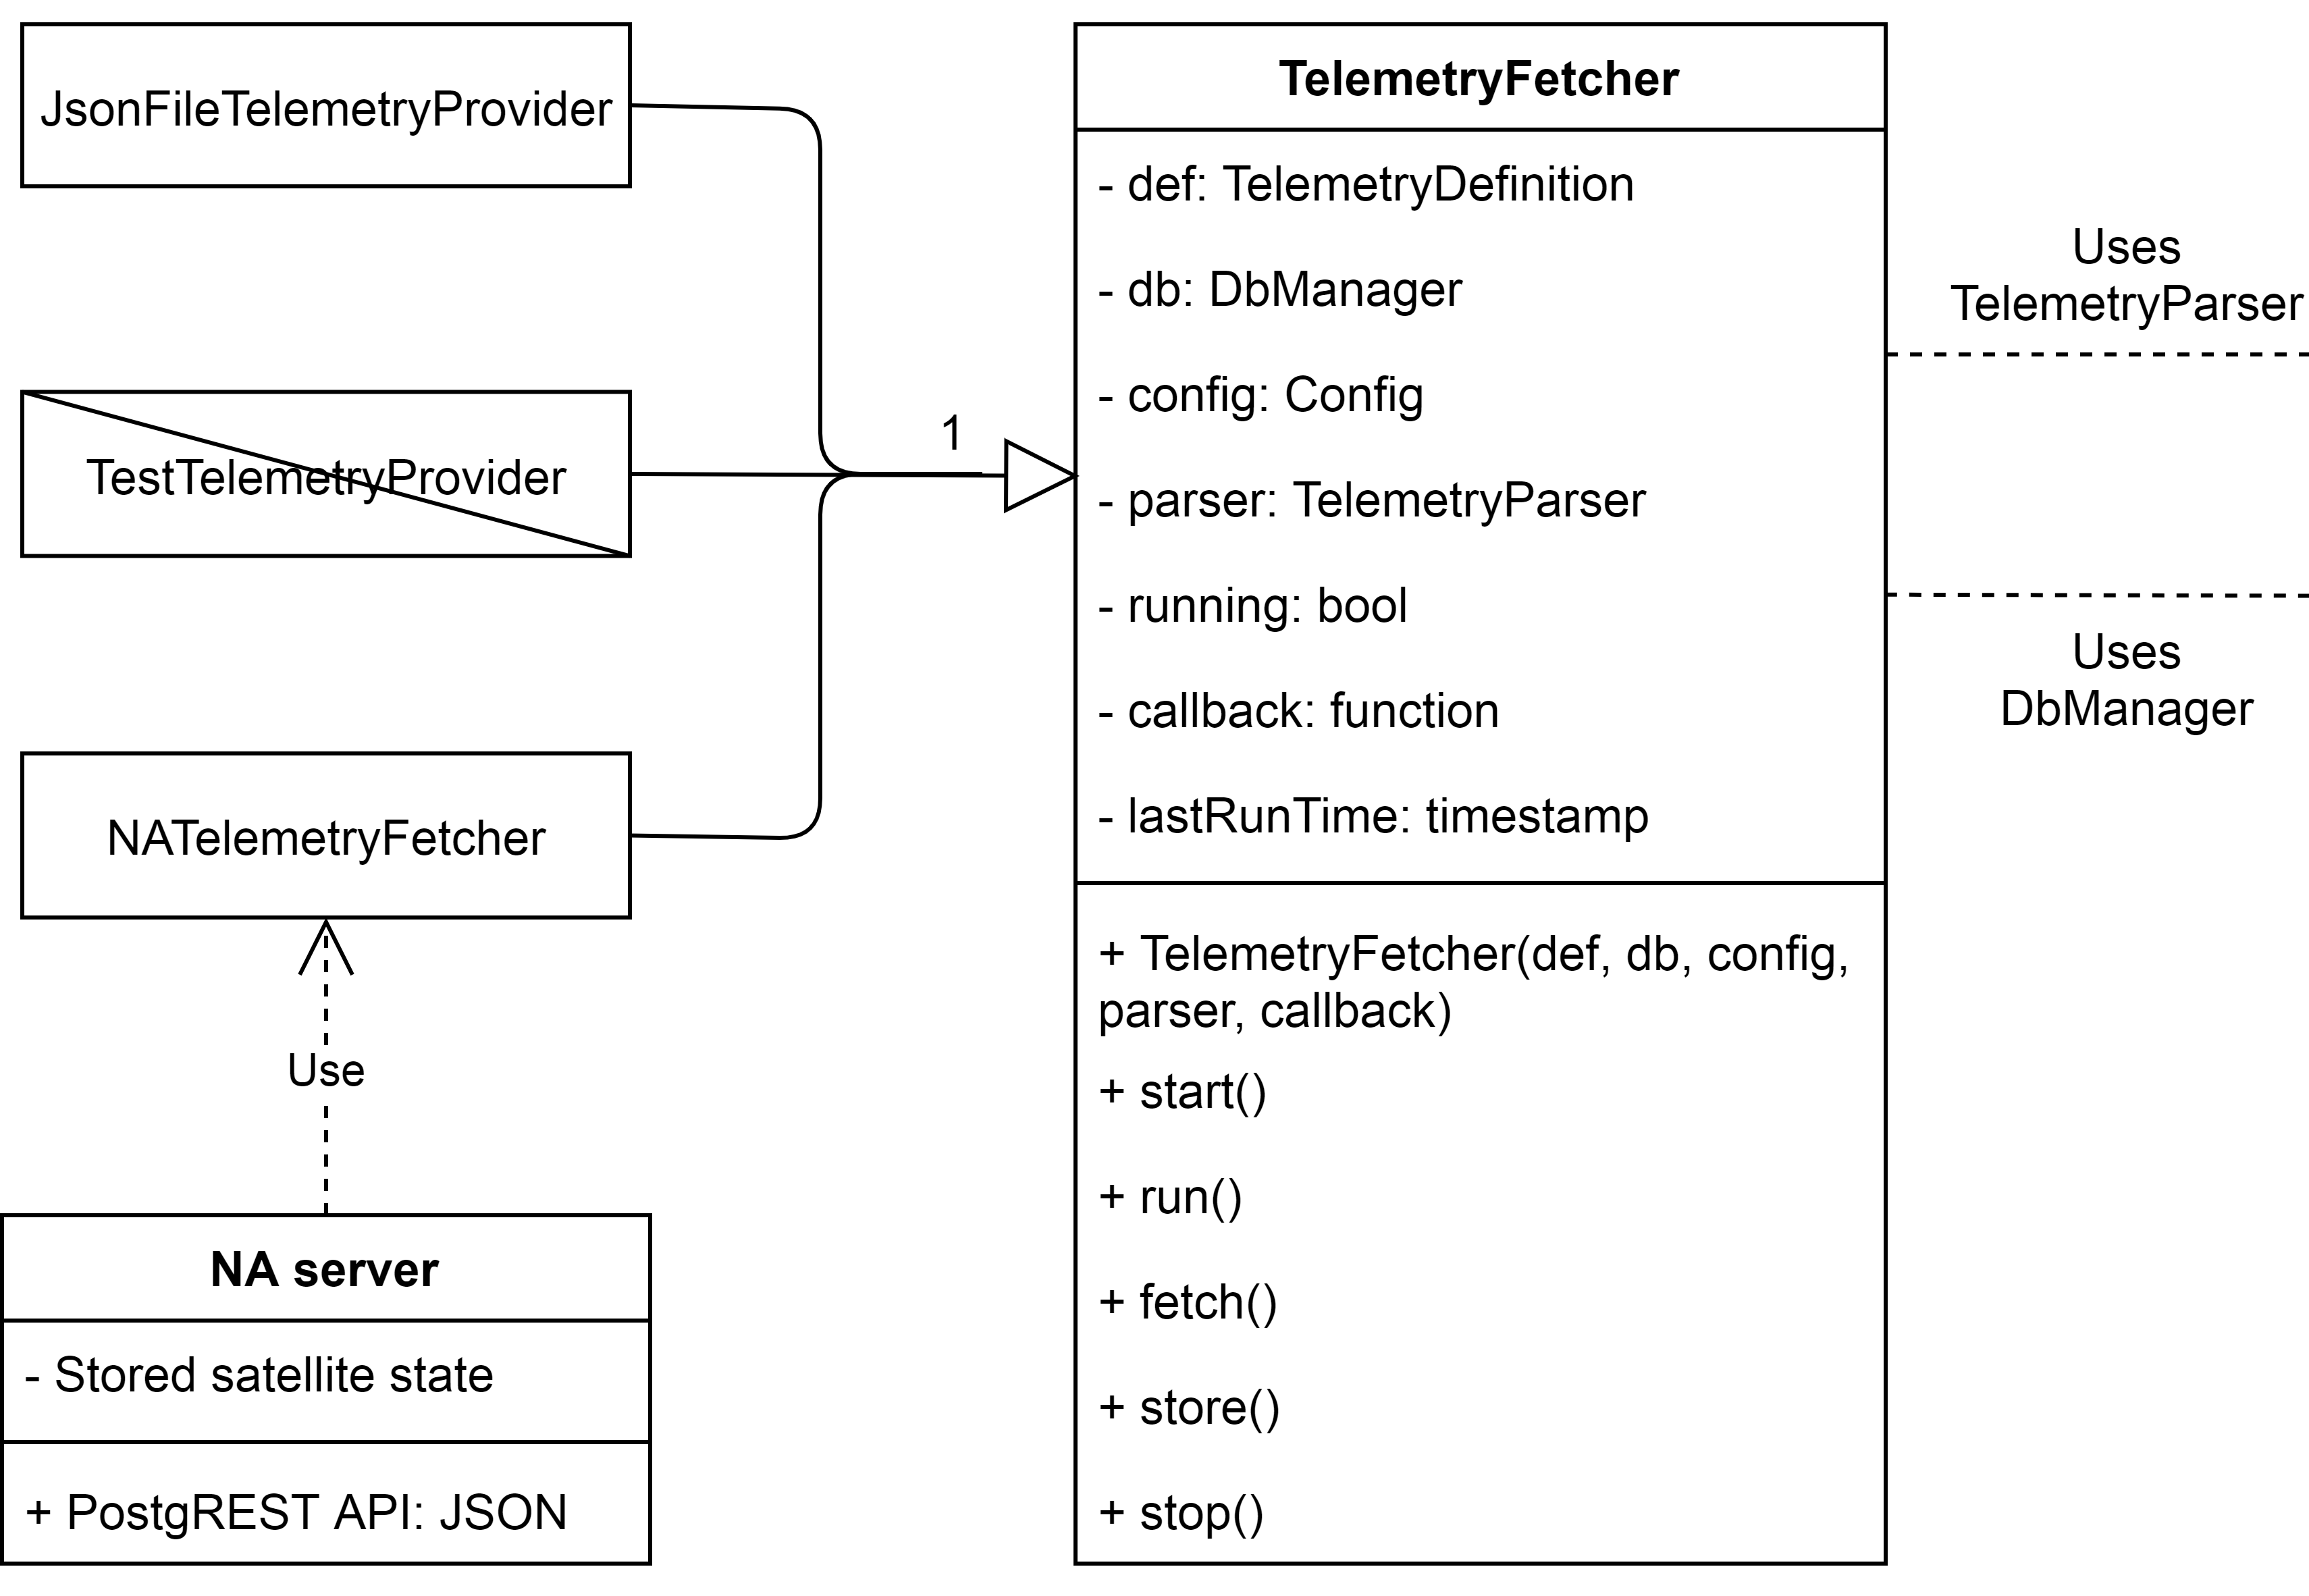
\includegraphics[width=0.7\linewidth]{Images/New Diagrams/TelemetryFetching.png}
  \caption{New Class Diagram: Telemetry Fetching}
  \label{fig:new_cdfetching}
\end{figure}

\subsubsection{Telemetry processing subsystem}
The main change is the addition of a new \inlinecode{parse(telemetryString)} method, which takes telemetry data directly from a fetcher and parses it to a valid telemetry object; this operation has no inverse, as the original telemetry string is included in this object and directly stored in the database in case it is required later, either due to changes in the definition requiring it to be parsed again or if another service than Open MCT needs access to a full copy of it. The field is also hashed and used to quickly check if an incoming telemetry sample already exists in the database.

Another new method is the \inlinecode{GetMctMetadata()} method, which returns a list of telemetry value metadata ready for use in Open MCT.

The updated class diagram for this subsystem can be found in Figure \ref{fig:new_cdparsing}.

\begin{figure}[H]
  \centering
  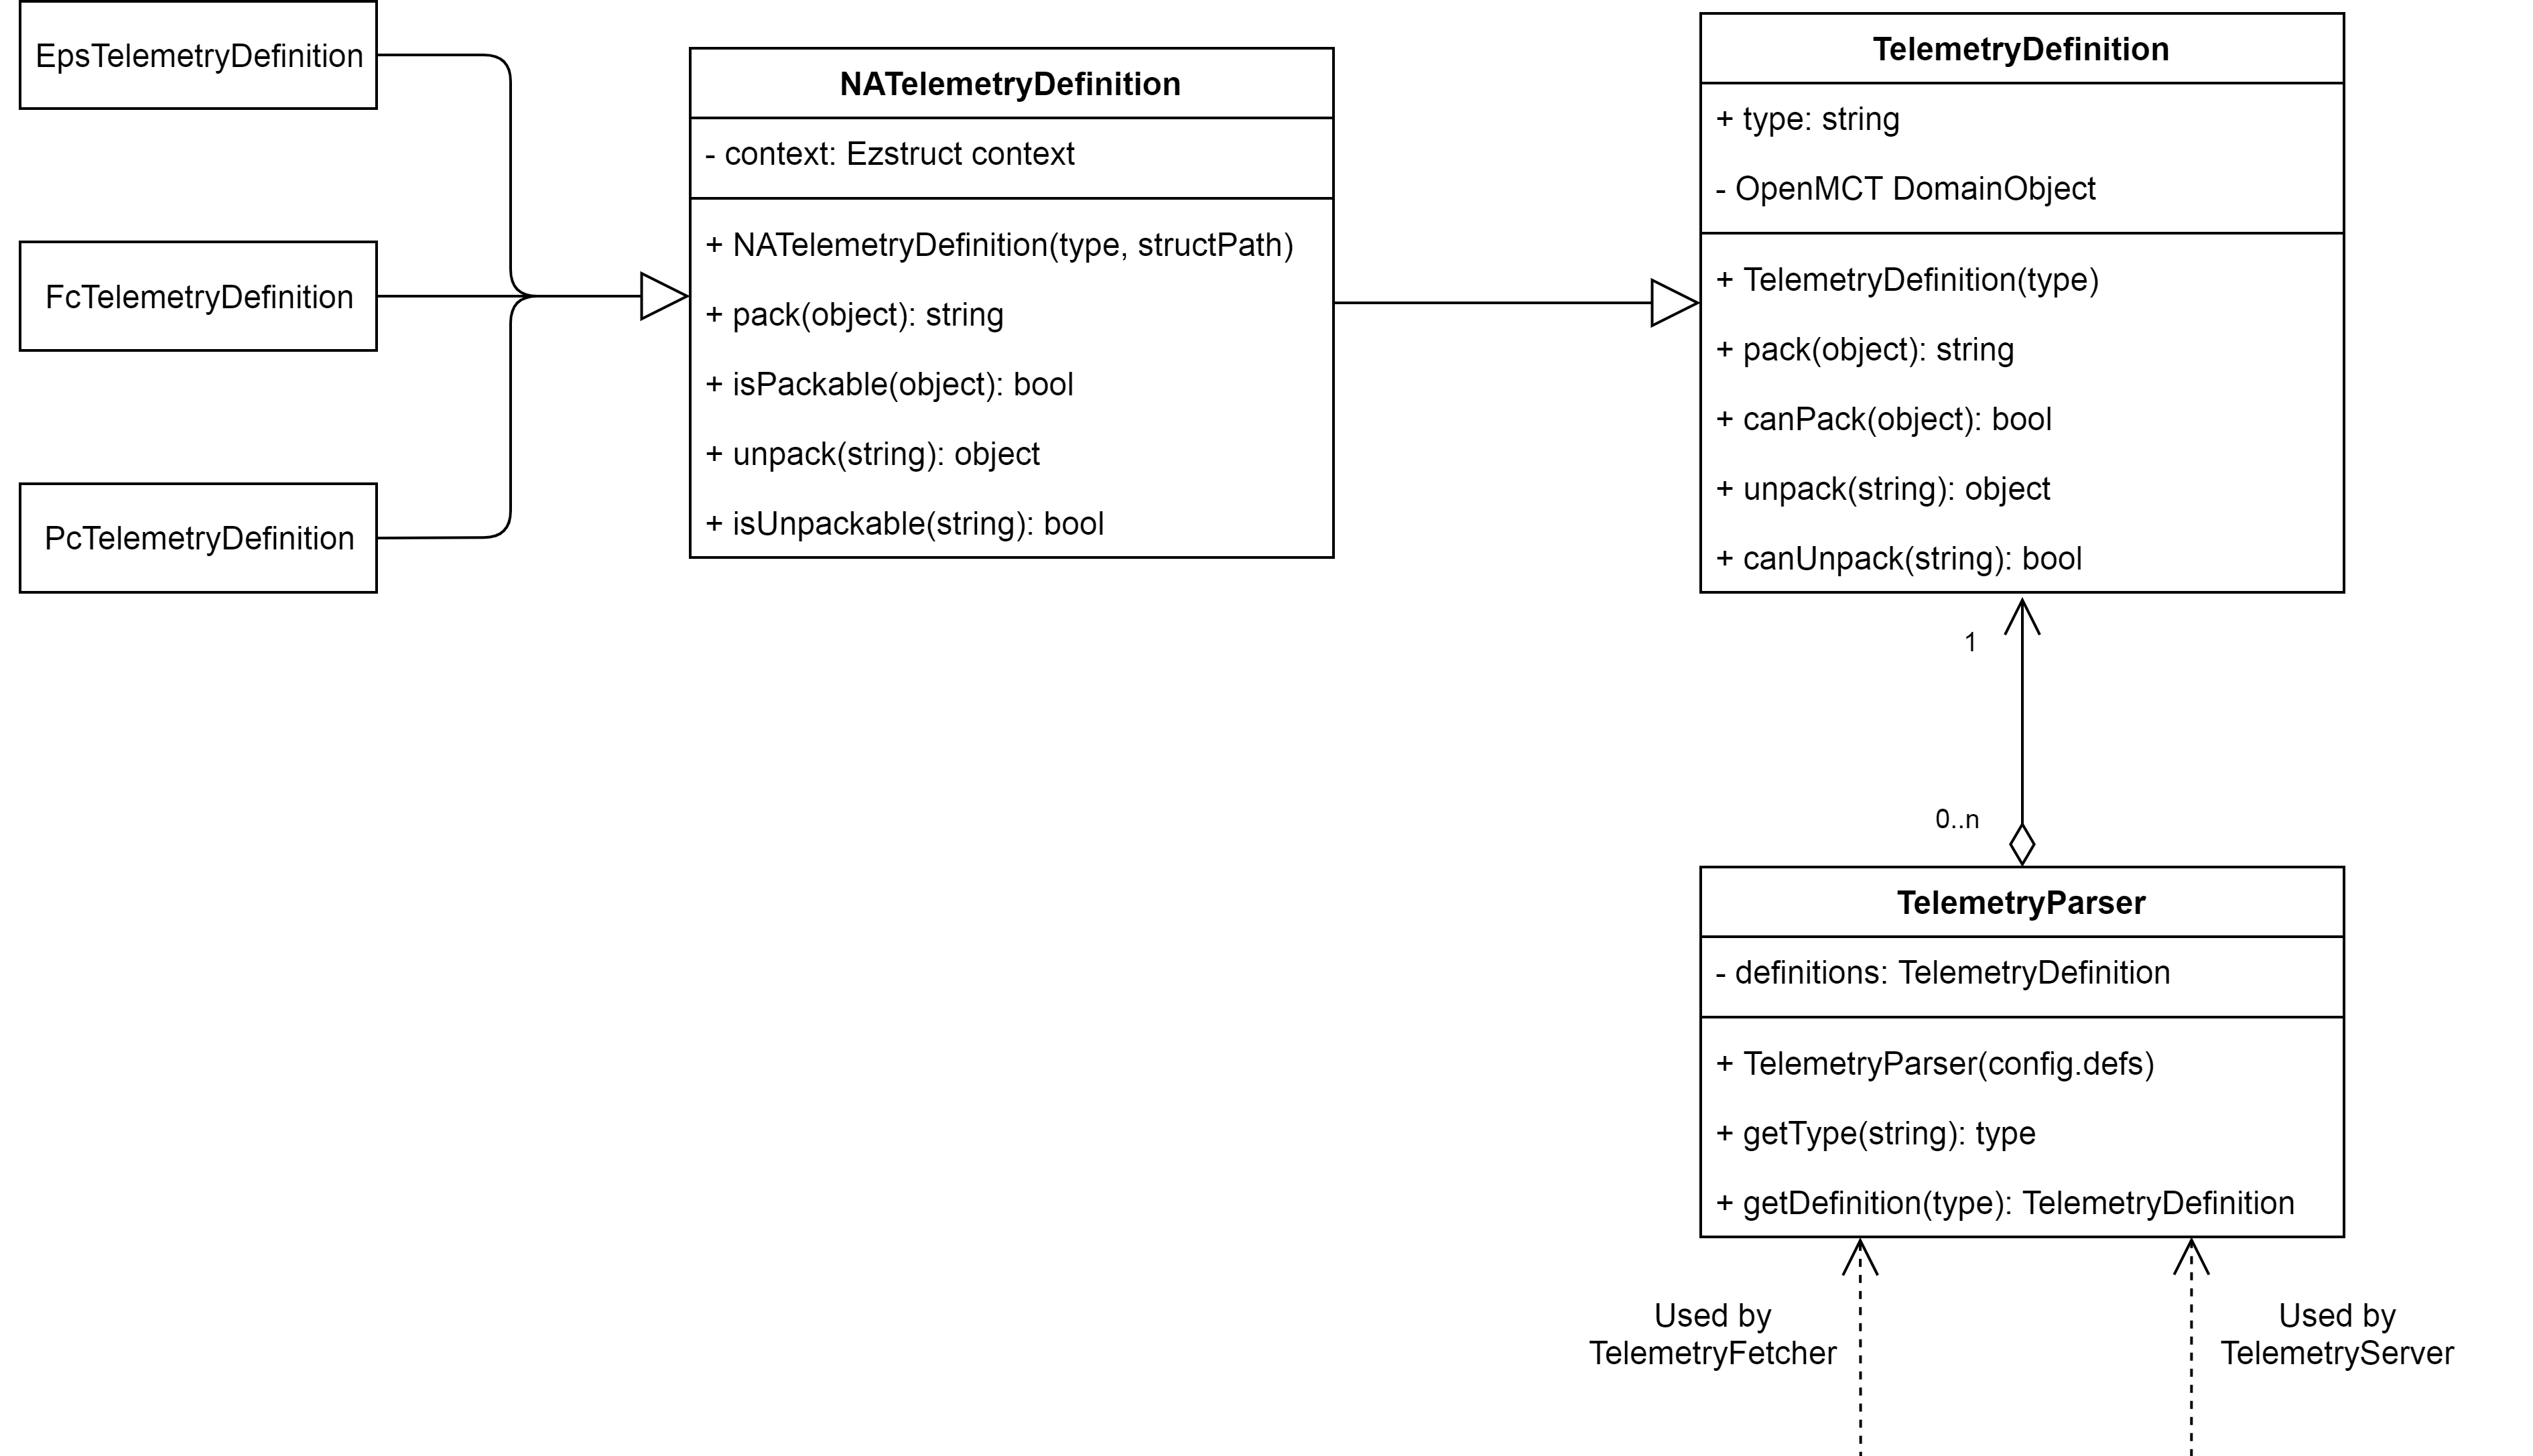
\includegraphics[width=1\linewidth]{Images/New Diagrams/TelemetryParsing.png}
  \caption{New Class Diagram: Telemetry Parsing}
  \label{fig:new_cdparsing}
\end{figure}

\subsubsection{Data management and storage subsystem}
The data management and storage subsystem needed fairly large changes to meet with the requirements (specifically \acrshort{fr}1.2, \acrshort{nfr}3.0 and \acrshort{nfr}4.0) due to very poor performance of the initially proposed architecture.

Especially the process of checking if a telemetry point was already stored in the database when running a \inlinecode{TelemetryFetcher} was very slow, resulting in system startup times with large \acrshort{json} inputs containing approximately 1000 telemetry points being on the order of multiple minutes (or worse). This could also lead to unacceptable performance with regards to the requirements on the response time of the system to incoming new data, since the system per now checks all inputs against the database to verify that they are new.

The solution to this was the implementation of a new column on the database table containing a SHA-1 \gls{hash} (chosen for its speed and fairly short length, see \cite{hashspeed}) of each stored telemetry point, generated using a new class called \inlinecode{DbHasher}. This column is used to create another index for the \inlinecode{Telemetry} table, eliminating the need to load and iterate over every single point in the database to check if a point already exists.

The performance gains from this change were fairly substantial, with \inlinecode{TelemetryFetcher} in many cases running multiple orders of magnitude faster. This was most noticeable with the \acrshort{eps} telemetry test dataset, which both had more points (18193 points vs. the 6719 points the \acrshort{fc} dataset) and about twice the byte length per telemetry point.

\begin{figure}[ht]
  \centering
  \includegraphics[trim=0 0 0 50, clip, width=0.9\linewidth]{Images/Graphs/Total load time.pdf}
  \caption{System startup: Total load time}
  \label{fig:perf_time}
\end{figure}

\begin{figure}[ht]
  \centering
  \includegraphics[trim=0 0 0 50, clip, width=0.9\linewidth]{Images/Graphs/Load time per telemetry point.pdf}
  \caption{System startup: Load time per telemetry point}
  \label{fig:perf_time_per_point}
\end{figure}

\begin{figure}[ht]
  \centering
  \includegraphics[trim=0 0 0 50, clip, width=0.9\linewidth]{Images/Graphs/Time spent in isPointNew.pdf}
  \caption{System startup: Percentage of load time spent in \inlinecode{isPointNew()}}
  \label{fig:perf_percentage}
\end{figure}

A comparison of the before/after performance of the data management and storage subsystem benchmarked using a \inlinecode{JsonFileTelemetryFetcher} at system startup can be found in figures \ref{fig:perf_time} to \ref{fig:perf_percentage}, with \say{\acrshort{db} init} referring to the case where the target database is empty.

The raw data used to create the performance graphs may be found in appendix A.

The updated class diagram for this subsystem can be found in Figure \ref{fig:new_cddb}.

\begin{figure}[H]
  \centering
  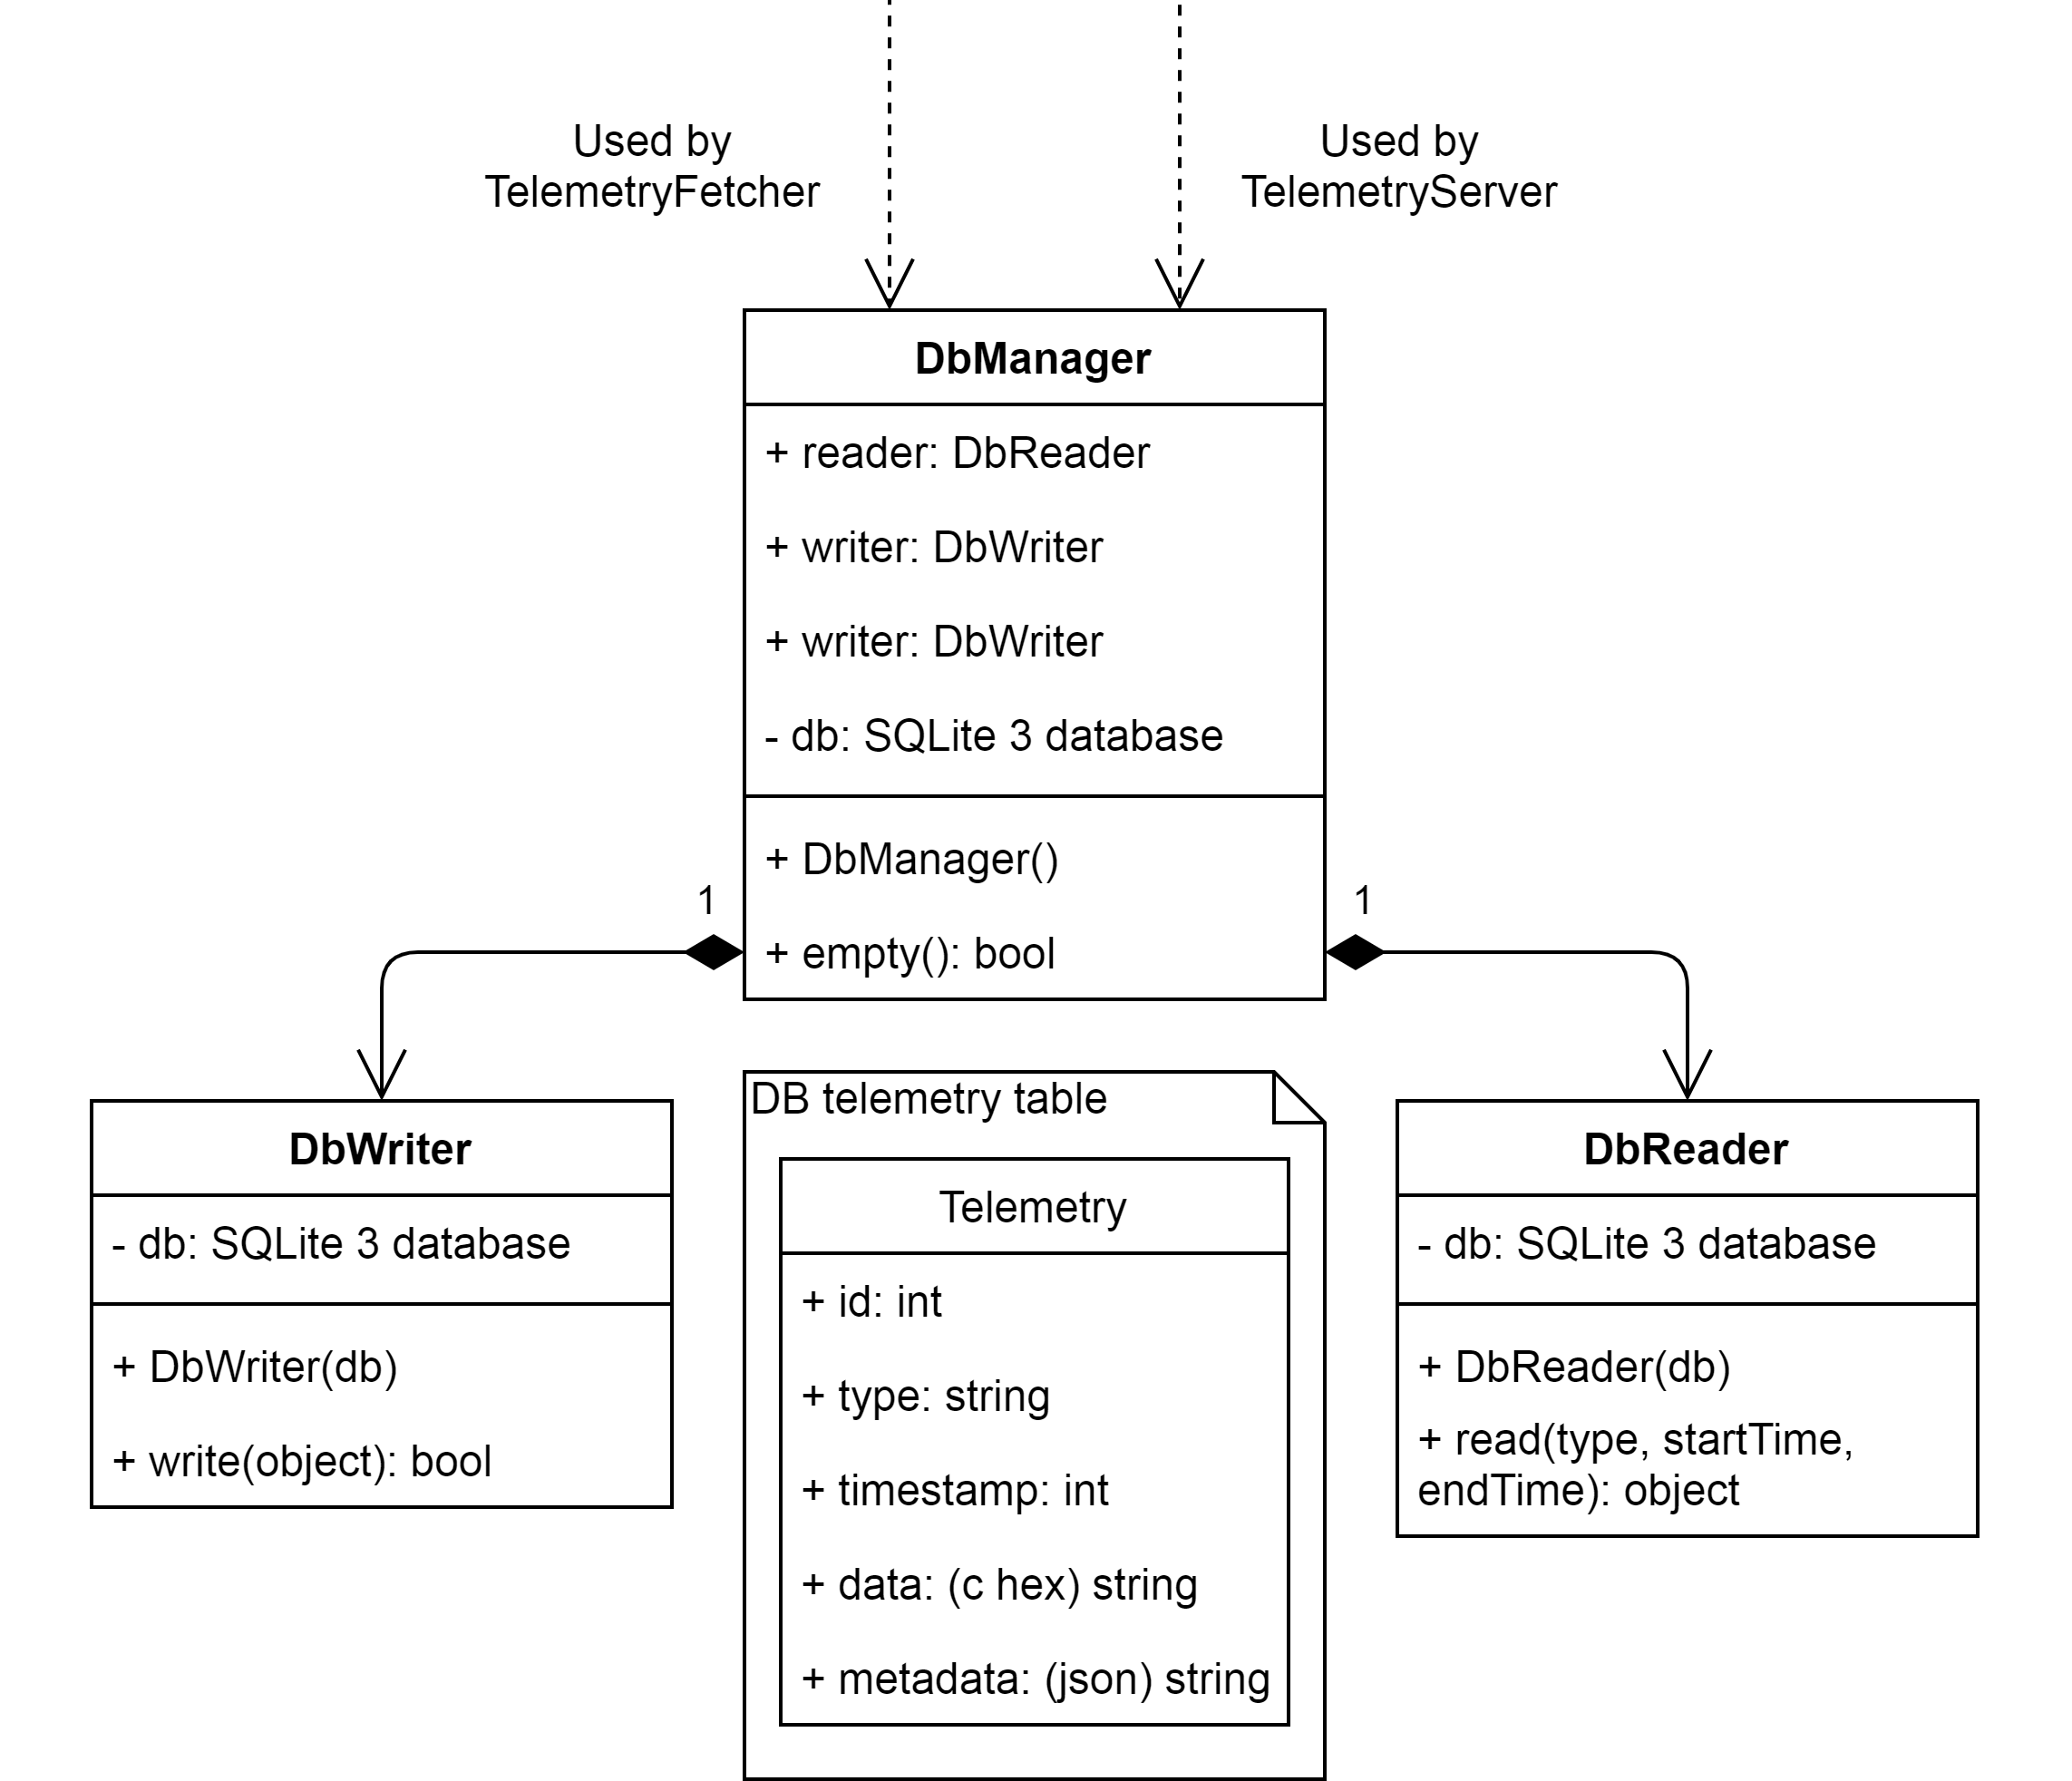
\includegraphics[width=0.65\linewidth]{Images/New Diagrams/DbManager.png}
  \caption{New Class Diagram: Database Management}
  \label{fig:new_cddb}
\end{figure}

\subsubsection{Telemetry serving subsystem}
The updated class diagram for this subsystem can be found in Figure \ref{fig:new_cdserving}. The main change here is the addition of the \inlinecode{ConfigServer} class, which provides system configuration from a \inlinecode{Config} instance and telemetry value metadata from \inlinecode{GetAllMctMetadata()} on a \inlinecode{TelemetryParser}.

\begin{figure}[H]
  \centering
  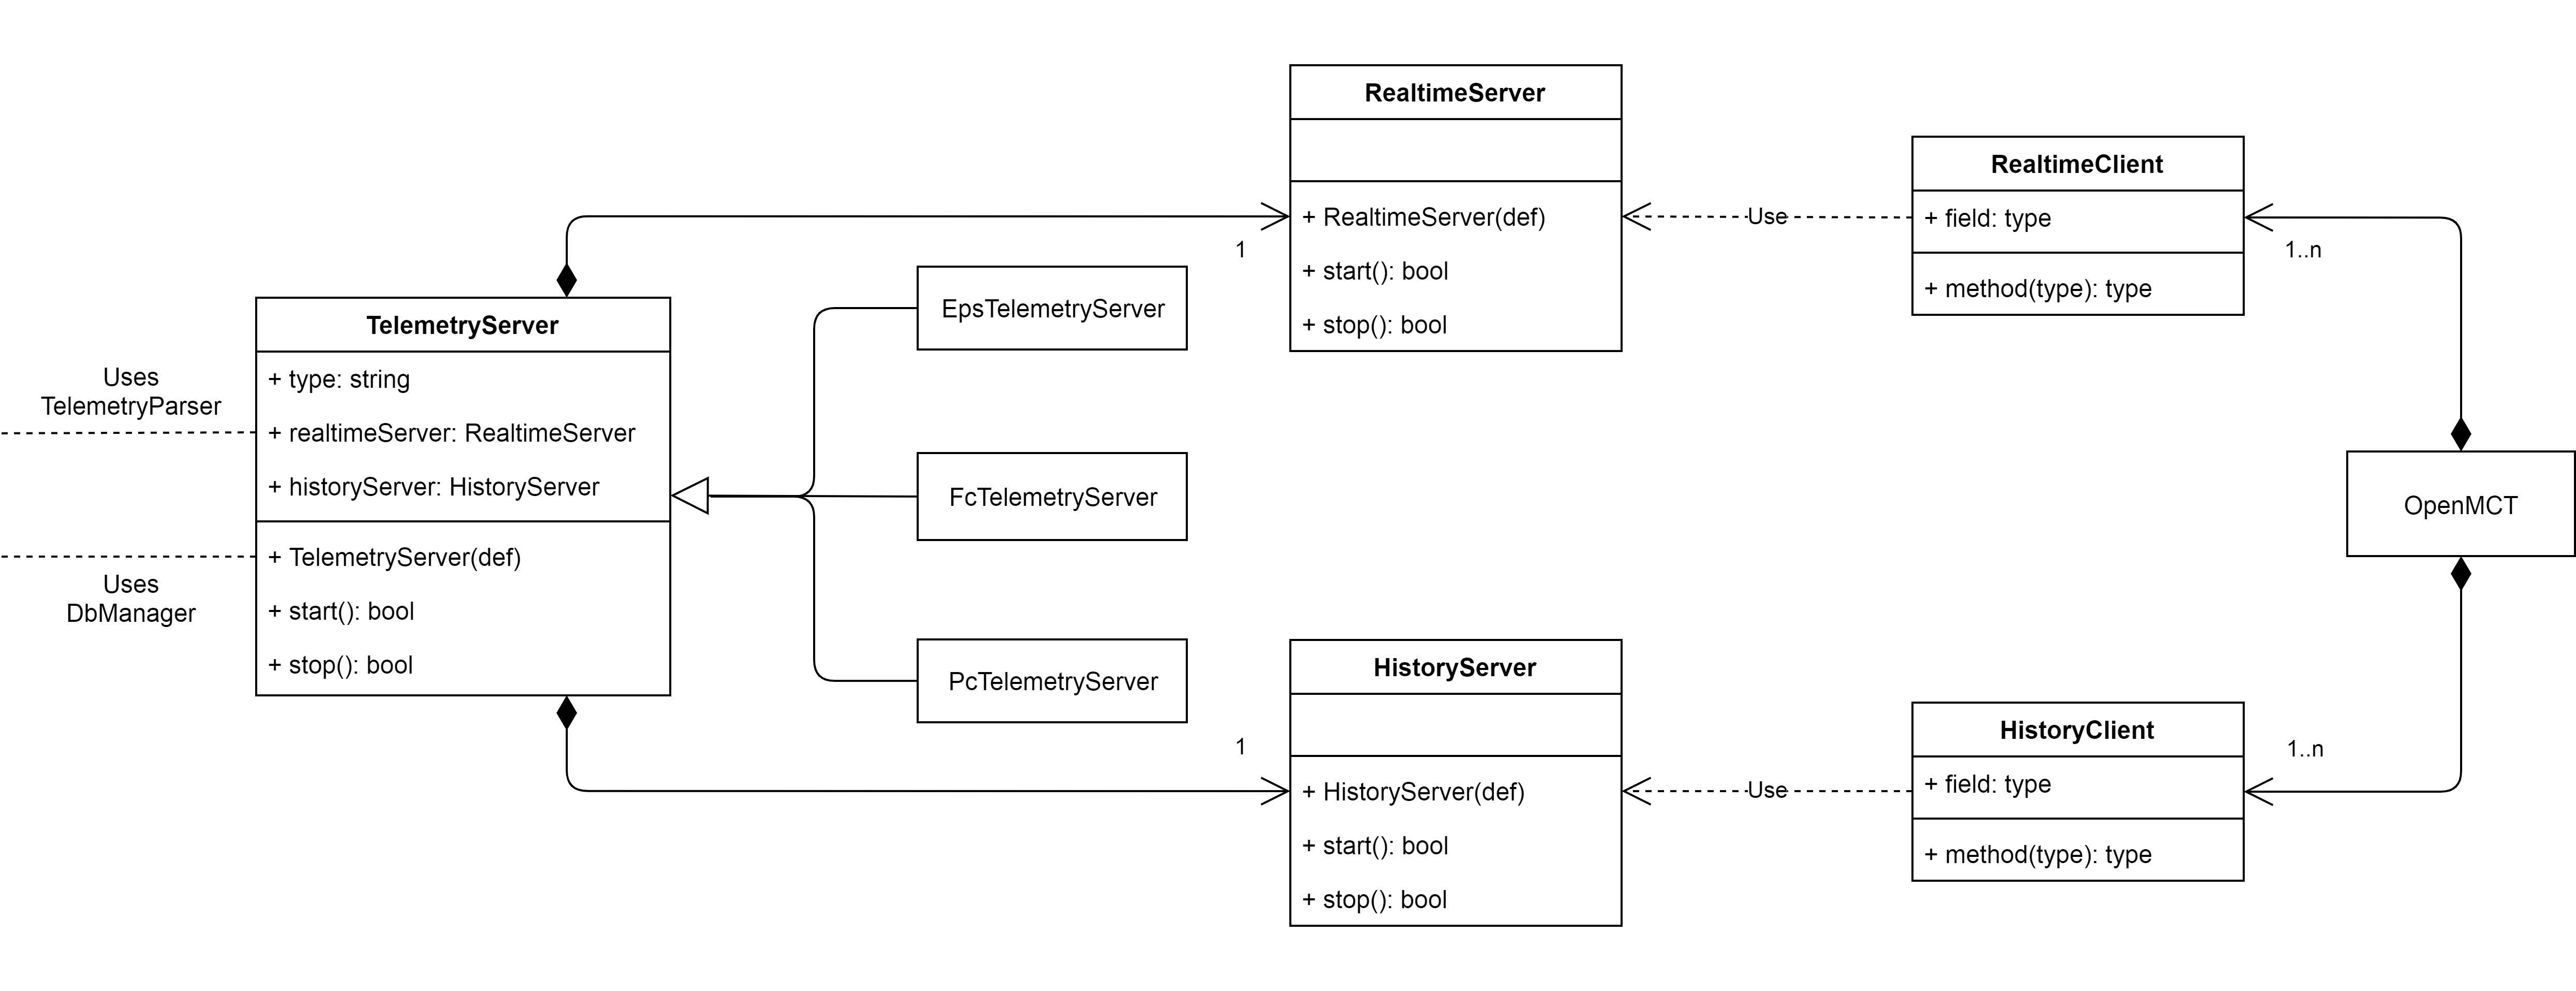
\includegraphics[width=1\linewidth]{Images/New Diagrams/TelemetryServing.png}
  \caption{New Class Diagram: Telemetry Server and Client}
  \label{fig:new_cdserving}
\end{figure}

\subsubsection{Open MCT client plugins}
These were underspecified in the initial system design proposal due to much of the implementation details being unknown, as with the telemetry serving subsystem that they connect to.

The final configuration has three plugins, with \inlinecode{ServerPlugin} being responsible for loading telemetry metadata from a \inlinecode{ConfigServer} and populating the Open MCT object tree (shown on the left-hand side in Figure \ref{fig:demoview}) with telemetry points. After this \inlinecode{RealtimeClient} and \inlinecode{HistoryClient} are loaded, which as the names imply connect to a \inlinecode{RealtimeServer} and \inlinecode{HistoryServer} respectively to provide telemetry data.

The updated class diagram for this subsystem can be found in Figure \ref{fig:new_cdserving}.

\subsection{Test coverage}
The test coverage requirements specified in \acrshort{nfr}7.0 were not quite met due to lack of time, but version 1.0 still has above $50\%$ unit test coverage for most files and metrics. The main hole in test coverage is for the Open MCT client plugins, due to them being finished last and functioning significantly different to all other parts of the system. Making good tests for them requires a significant level of insight into how Open MCT works.

A short summary of the system's test coverage may be found in table \ref{tab:tests}, with a full \Gls{jest} test coverage report available in appendix B.

\begin{table}[ht]
\centering
\caption{System Test Coverage Summary}
\label{tab:tests}
\begin{tabular}{|l|l|l|l|l|}
\hline
\rowcolor[HTML]{C0C0C0} 
File or directory     & Statements & Branches & Functions & Lines  \\ \hline
All files             & 68.4\%     & 50.4\%   & 56.1\%    & 68.2\% \\ \hline
Plugins               & 15.9\%     & 45.0\%   & 4.76\%    & 16.1\% \\ \hline
Telemetry definitions & 77.0\%     & 62.8\%   & 62.16\%   & 76.4\% \\ \hline
Web server            & 61.1\%     & 11.1\%   & 66.7\%    & 61.1\% \\ \hline
Database              & 69.9\%     & 31.3\%   & 69.6\%    & 70.3\% \\ \hline
Telemetry services    & 75.5\%     & 75.0\%   & 60.4\%    & 75.1\% \\ \hline
\end{tabular}
\end{table}

% The \Gls{latex} typesetting markup language is specially suitable for documents that include \gls{maths}. 